\sys is a new programming and execution model for intermittent computing on energy-harvesting devices. \sys addresses the challenges outlined in Section~\ref{sec:background} to make task-based intermittent programs {\em programmable} and {\em efficient}. \sys accomplishes this goal with a constellation of a new programming model and run time software system support, that supports dynamically adaptive task-based execution. Figure~\ref{fig:system_overview} shows an overview of \sys.

\begin{wrapfigure}{t!}{0.5\textwidth}
	\centering
	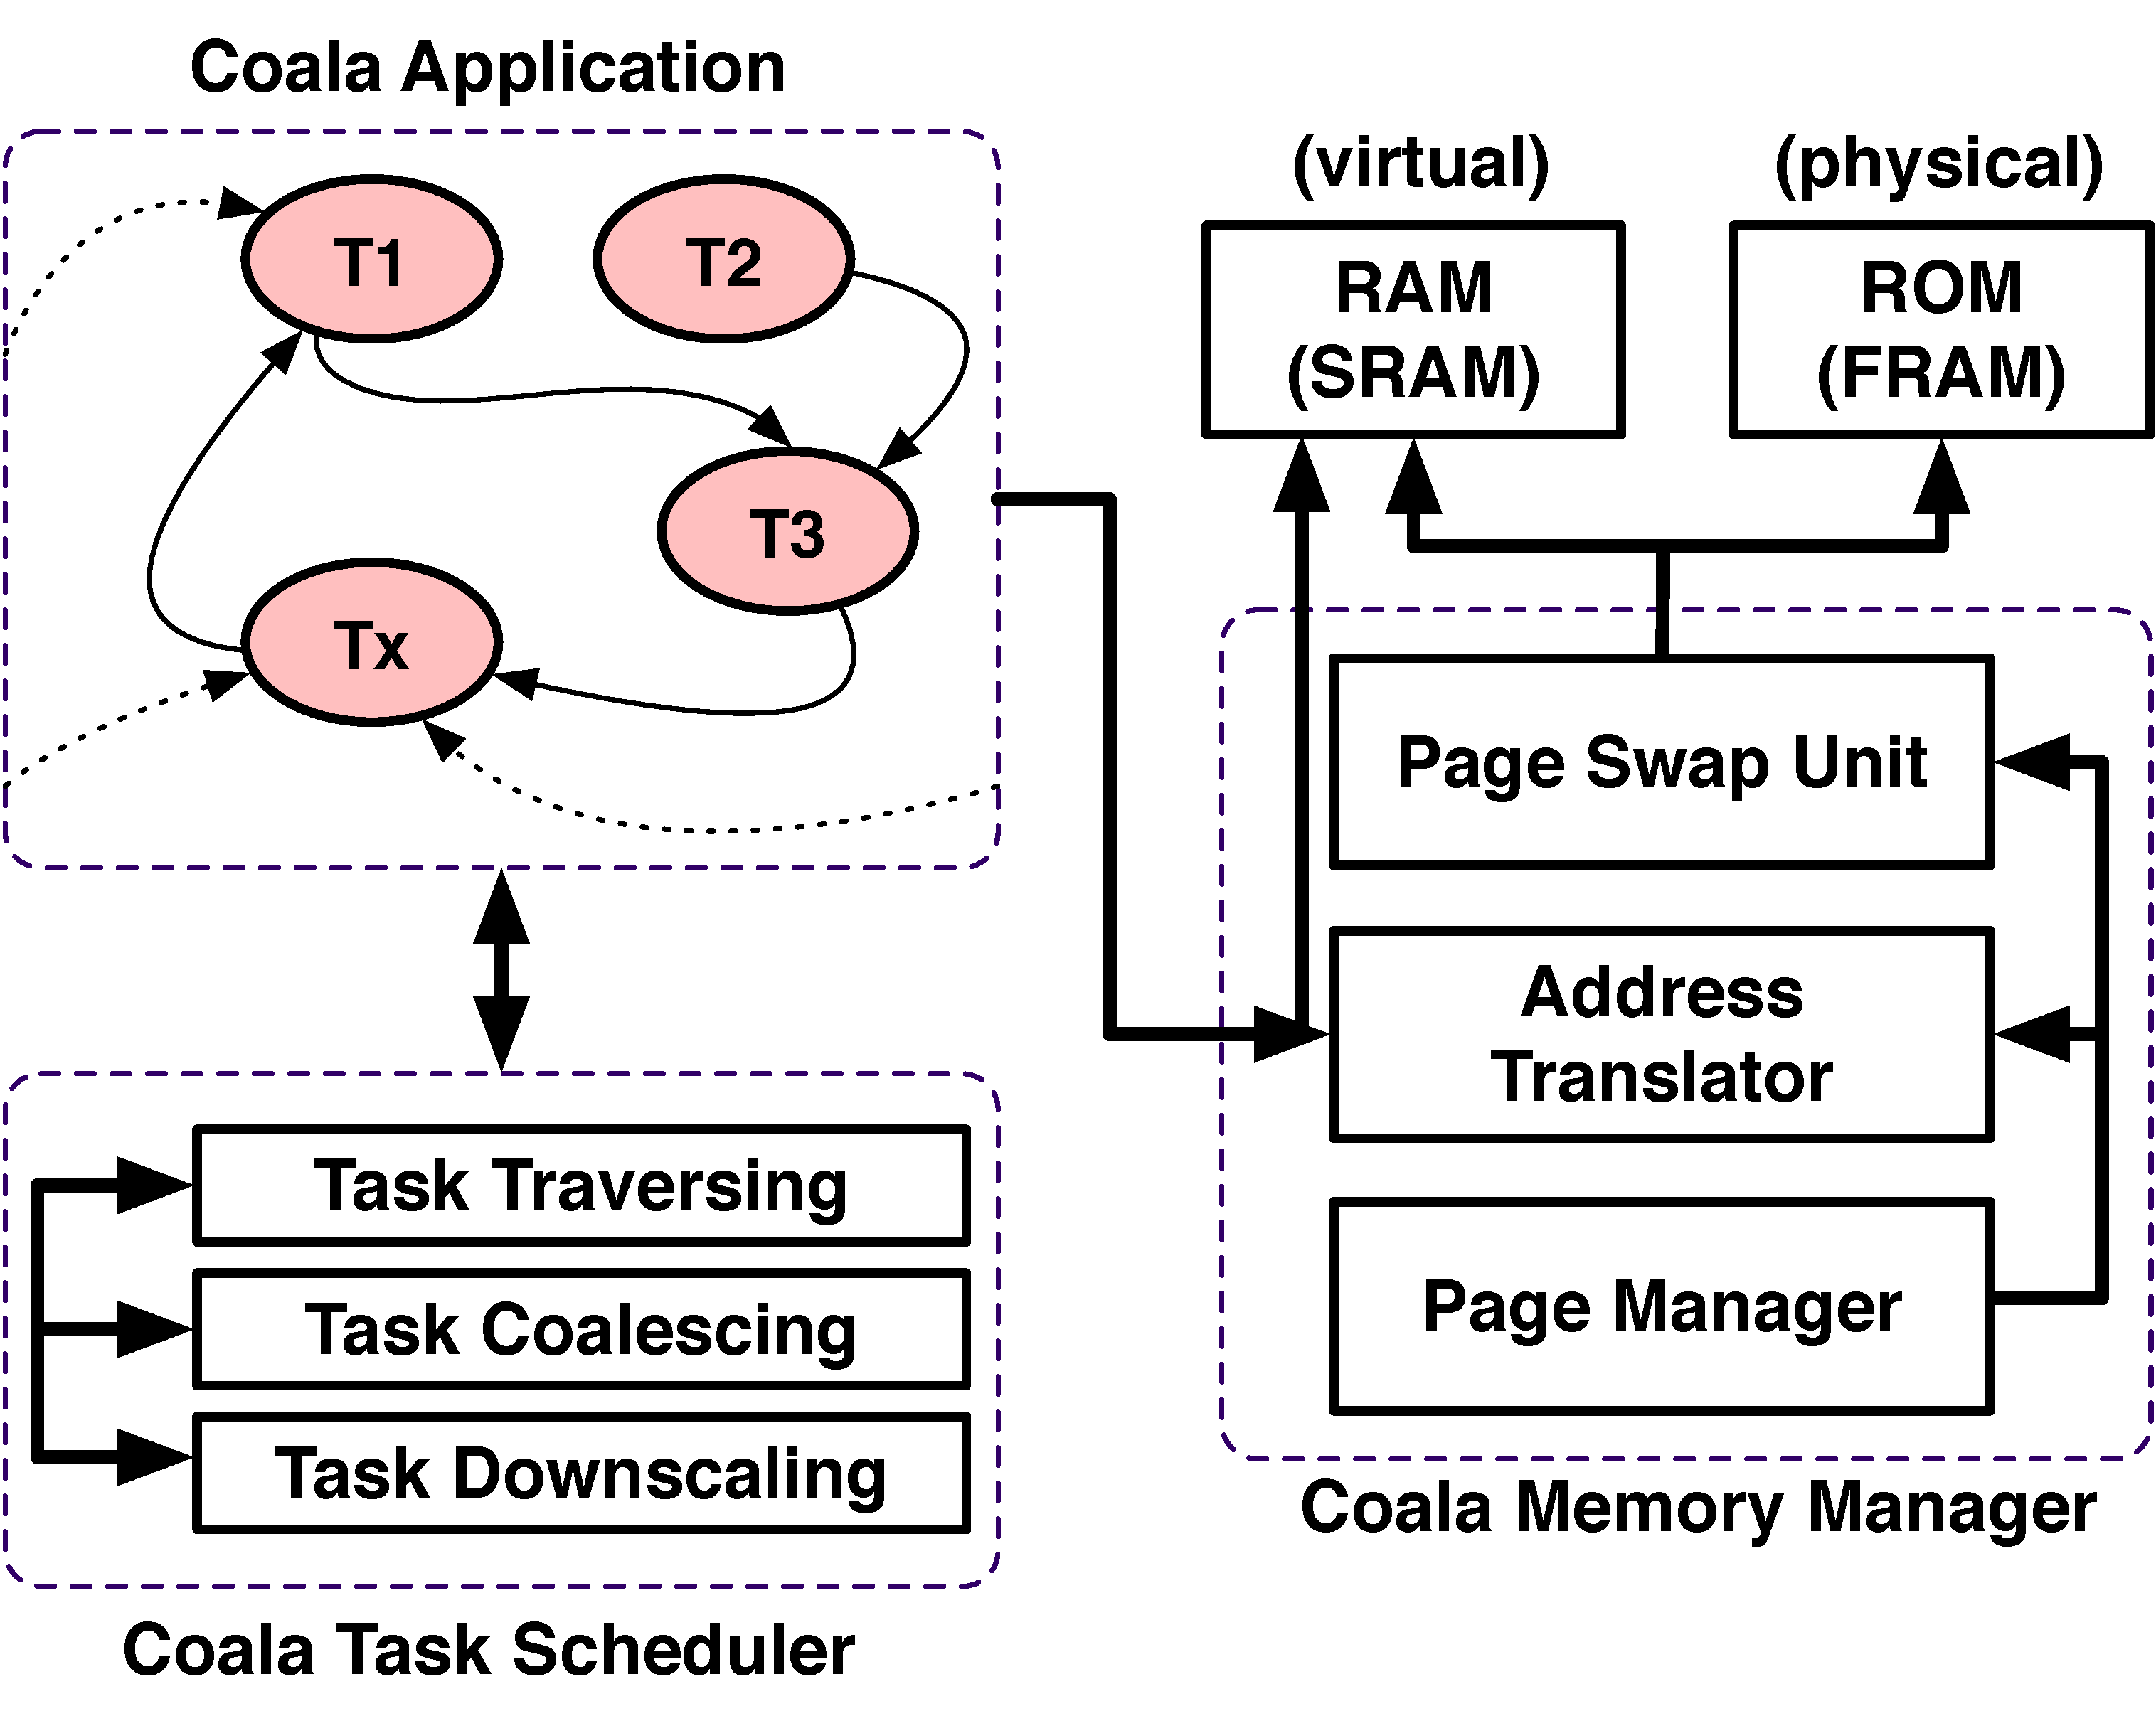
\includegraphics[width=0.5\columnwidth]{figures/graffle/overview.pdf}
	\caption{\sys top-level view. \textcolor{red}{redraw the figure: change font type}}
	\label{fig:system_overview}
\end{wrapfigure}

\textbf{\sys Programming and Execution Model.}  To use \sys, a programmer first writes plain, imperative C code. The programmer then must decompose the program into tasks. To manually decompose a program into tasks, the programmer designates a set of functions as tasks, sequences control-flow between these tasks, and annotates memory accesses that manipulate data shared by multiple tasks. In other words, it requires reasoning similar to prior task-based systems~\cite{chain,alpaca}. 

A programmer may also opt to use compiler support to automatically decompose a program into tasks, leveraging recent work~\cite{cleancut_2018,baghsorkhi_cgo_2018}. Without loss of generality, we assume throughout this work that the programmer manually decomposed the program into tasks; \sys's behavior with automatically decomposed code would be identical.

The programmer compiles their task-based code, and links to the \sys runtime, producing a \sys-enabled binary. The \sys runtime implements \sys's task-based programming and execution model. The runtime system also includes \sys's novel {\em virtualizing memory manager} and its {\em task coalescing manager}, and {\em task downscaling manager}, both of which are essential to \sys's adaptive task-based execution.

\textbf{\sys Task Coalescing Manager.} \sys relies on its task coalescing manager to dynamically {\em coalesce} statically\hyp{}defined tasks to avoid inessential overheads associated with completing tasks. By default, tasks run in a sequence and each task commits its task-shared state as it completes.  The time and energy cost of a task's commit is unnecessary if the task and its successor both complete without a power failure. The key insight that \sys leverages is that the first task could have deferred its commit to the second task. {\em coalescing} tasks by deferring the first commit avoids the fixed cost of the first commit (task transitioning overheads). Coalescing also amortizes per-variable commit cost, committing each location accessed by both tasks only after the second task, rather than once per task. Details of coalescing are presented in Section~\ref{sec:task_coalescing}.

\textbf{\sys Task Downscaling Manager.} Details of task downscaling are presented in Section~\ref{sec:task_downsizing}. \textcolor{red}{to be written}
 
\textbf{\sys Virtual Memory Manager.} \sys is able to efficiently coalesce tasks because of its efficient virtual memory manager, which is described in Section~\ref{sec:memory_virtualization}. \sys's memory manager paginates memory and ensures that data in a page remain consistent despite power interruptions. \sys allows a task to manipulate data in a volatile copy of a page only. Pages swap between volatile and non-volatile memory, depending on the capacity of the volatile memory and the program's access pattern. \sys tracks a task's memory accesses efficiently at page granularity (rather than using, e.g., costly word-granular tracking). When a task ends, each page it accessed commits from volatile memory (or from a non-volatile swap region for dirty pages) back to the non-volatile main memory. Pages efficiently, atomically commit using a two-phase commit procedure accelerated using hardware support for direct memory access (DMA). Details of Virtual Memory Manager are presented in Section~\ref{sec:memory_virtulaization}.